\section{Arquitetura do Software}

O objetivo dessa seção é apresentar e detalhar a arquitetura que foi utilizada na plataforma PGTBL. O desenvolvedor que
ler essa seção obterá uma visão geral de como esse software está estruturado.

\subsection{Representação Arquitetural}

O projeto será implementado utilizando o framework Django na versão 2.0. O django utiliza-se do MVT (Model-View-Template) como uma adaptação do MVC (Model-View-Controller), nas views utilizaremos as \textit{Class Based Views} para padronização do código. Esse framework fará comunicação com o banco de dados Postgresql e o servidor nginx.  A figura \ref{fig:arquitetura} exemplifica essa representação arquitetural.

\begin{figure}[h!]
	\centering
  \includegraphics[keepaspectratio=true,scale=0.4]{figuras/arquitetura.eps}
  \caption[Representação Arquitetural.]{Representação Arquitetural. Fonte: Autor}
	\label{fig:arquitetura}
\end{figure}

\begin{enumerate}
  \item O web client (navegador) manda uma requisição para o web server (Nginx) com o protocolo HTTP.
  \item Os arquivos estáticos armazenados no sistema de arquivos, como CSS, JavaScript, Imagens e documentos PDF,
    podem ser processados diretamente pelo web server (Nginx).
  \item A parte dinâmica é delegada ao servidor de aplicativos WSGI (Web Server Gateway Interface) do django, no caso
    o gunicorn que é um servidor WSGI para Unix feito em python puro, ele irá converter solicitações HTTP recebidas
    do servidor em chamadas python em colaboração com o framework django que irá ter um arquivo chamado urls.py que
    diz ao nginx qual código deverá ser executado de acordo com o path e código HTTP recebido, através de proxy
    reverso será feito o redirecionamento inicial do Nginx com o servidor da aplicação, ou seja, o proxy reverso
    irá funcionar como uma ponte de ligação entre o nginx e o django através do gunicorn.
  \item Dentro do django a requisição recebida pelo web server é mapeado para uma view especifica através das urls,
    a view pede dados a modelo, a model pega os dados do banco de dados postgresql e retorna a view, esta seleciona
    o template e fornece os dados, com isso o template é preenchido e devolvido a view que devolve o template como
    resposta ao web server.
  \item O web server (nginx) retorna a resposta para o web client (navegador)
\end{enumerate}

\subsection{Pacotes Significativos do Ponto de Vista da Arquitetura}

A figura \ref{fig:pacotes} lista todos os pacotes do ponto de vista da arquitetura do software.

\begin{figure}[h!]
	\centering
  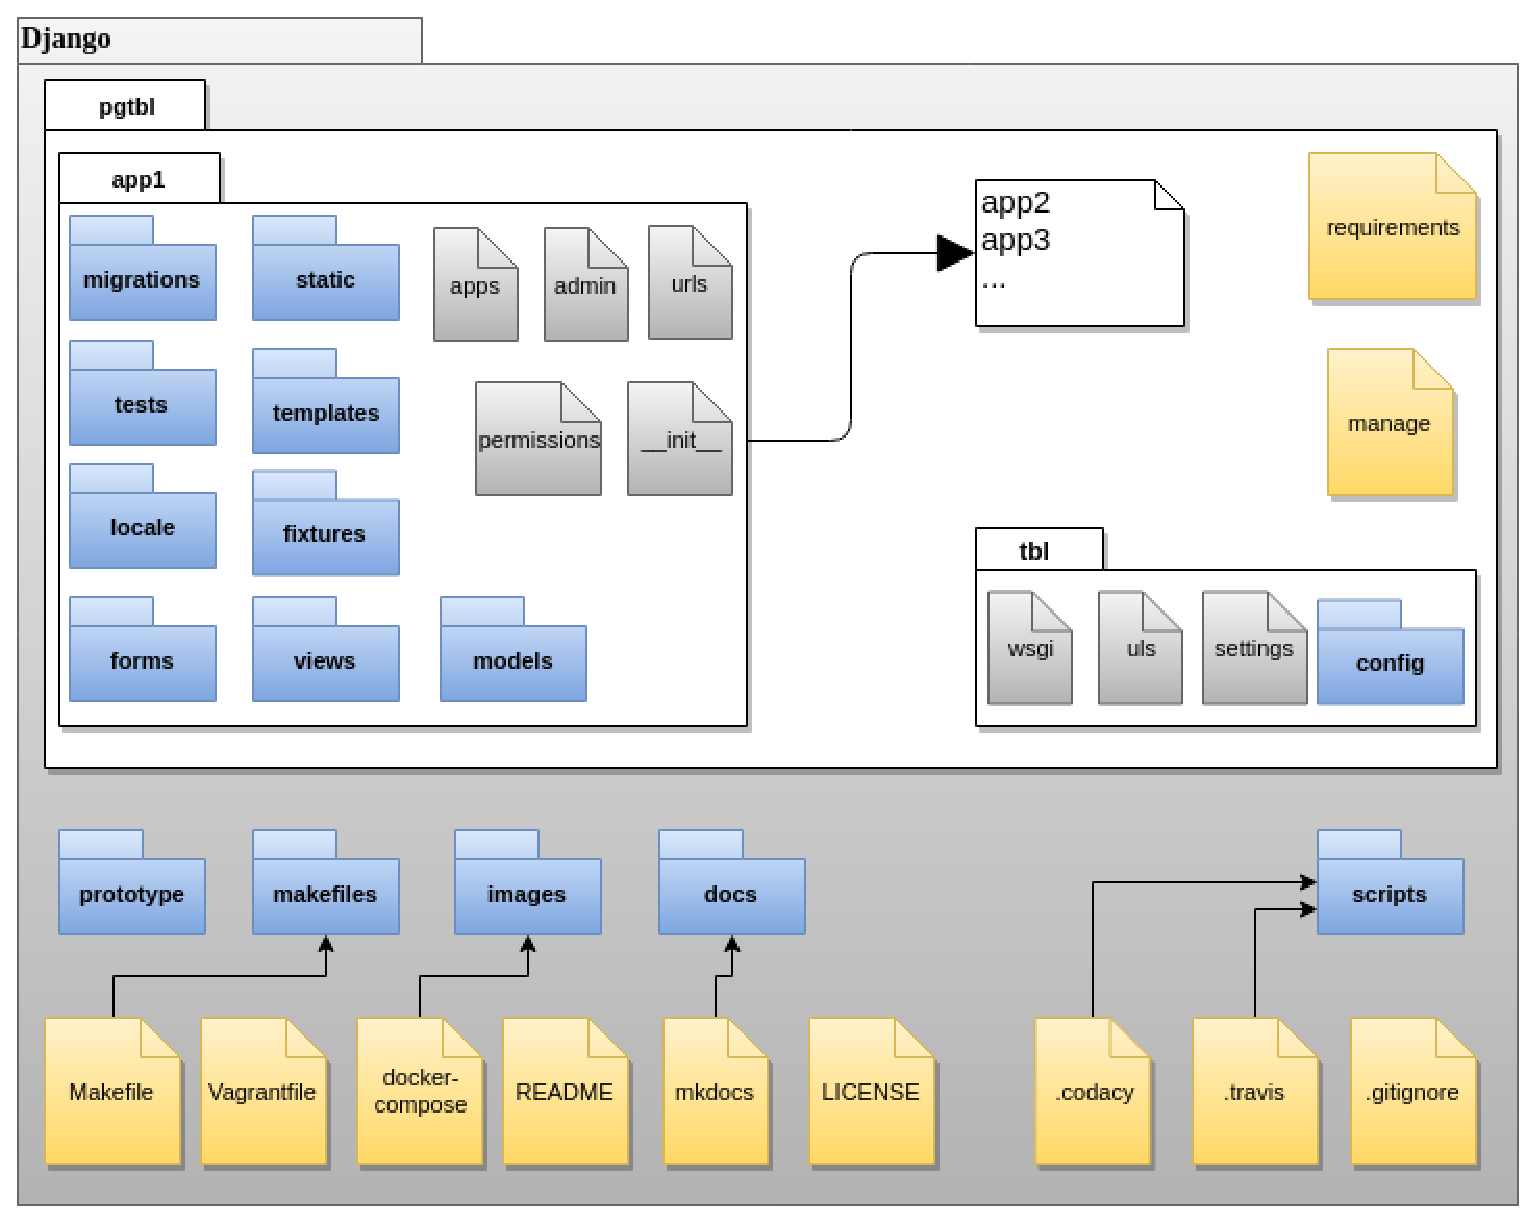
\includegraphics[keepaspectratio=true,scale=0.5]{figuras/pacotes.eps}
  \caption[Pacotes do projeto.]{Pacotes do projeto. Fonte: Autor}
	\label{fig:pacotes}
\end{figure}

\begin{itemize}
  \item Os pacotes de cada aplicação:
  \begin{itemize}
    \item \textbf{locale}: Pasta que irá ter toda a tradução do software para pt-BR.
    \item \textbf{migrations}: pasta com todas as migrações das modelos para o banco, são os SQLs.
    \item \textbf{static}: É onde fica os arquivos estáticos da aplicação (CSS, JS e IMG)
    \item \textbf{templates}: É onde fica os templates da aplicação (HTML)
    \item \textbf{tests}: contém os testes automatizados feitos no sistema.
    \item \textbf{\_\_init\_\_}: É o arquivo que define que sua pasta é um pacote python.
    \item \textbf{admin}: contém a instância da modelo que fará parte do sistema de administração do django.
    \item \textbf{app}: arquivo que contém informações da aplicação do django.
    \item \textbf{forms}: pasta que contém os campos que será inserido no formularios
    \item \textbf{models}: pasta de arquivos que faz interface com o banco de dados, é responsável por leitura,
      validação e escrita de dados no banco de dados.
    \item \textbf{permissions}: Arquivo de implementação de permissões do aplicativo.
    \item \textbf{urls}: São as rotas para ser acessada pelo navegador
    \item \textbf{views}: pasta que contém a camada lógica do sistema e a comunicação com o navegador por meio de
      rotas (Classe Based Views).
    \item \textbf{fixtures}: pasta que contém arquivos json para pré-popular o banco de dados para testes manuais
  \end{itemize}
  \item Os pacotes de configuração:
  \begin{itemize}
    \item \textbf{config}: É uma pasca que contém as configurações do software separada em arquivos.
    \item \textbf{settings}: São as configurações gerais do software importadas da pasta config.
    \item \textbf{urls}: Arquivo que terá o mapeamento de rotas de todo o projeto com todas as aplicações.
    \item \textbf{wsgi}: Arquivo usado para deploy do projeto.
  \end{itemize}
  \item Os pacotes do projeto Django:
  \begin{itemize}
    \item \textbf{manage}: Arquivo de configuração geral do django.
    \item \textbf{requirements}: Arquivos para instalar dependências da aplicação através do seguinte comando:
      pip3 install -r requirements.txt
  \end{itemize}
  \item Os pacotes gerais do projeto PGTBL:
  \begin{itemize}
    \item \textbf{Vagrantfile}: Arquivo que gerencia a máquina virtual de desenvolvimento, criado para desenvolvedores
      que queiram desenvolver em sistemas operacionais diferentes do Linux, como Windows ou Mac, precisa ter o
      Vagrant instalado.
    \item \textbf{Makefile}: Arquivo de atalhos para comandos muito usados pelos desenvolvedores.
    \item \textbf{docker-compose}: Arquivos que gerencia todos os containers da aplicação
      (deploy, homolog, production, test e desenvolvimento).
    \item \textbf{.travis}: Arquivo que gerencia a entrega continua da aplicação através da ferramenta Travis CI no github.
    \item \textbf{.codacy}: Arquivo de configuração da ferramenta de análise estática de código Codacy.
    \item \textbf{.gitignore}: Arquivo que faz o git ignorar alguns arquivos do projeto.
    \item \textbf{README}: Arquivo com um conteúdo markdown inicial do projeto.
    \item \textbf{LICENSE}: Licença do software.
    \item \textbf{mkdocs}: Arquivo que contém a configuração da documentação do software.
    \item \textbf{prototype}: Pasta com o protótipo do software.
    \item \textbf{docs}: Pasta com toda a documentação do software.
    \item \textbf{makefiles}: Pasta que contém de forma organizada comandos do Makefile.
    \item \textbf{images}: Pasta que armazena as imagens de deploy da aplicação tbl.
    \item \textbf{scripts}: Pasta com alguns scripts de integração e deploy continuo
  \end{itemize}
\end{itemize}

O repositório com o código fonte do projeto se encontra no seguinte link: \url{https://github.com/VictorArnaud/PGTBL}

\subsection{Diagrama de Classe}

O diagrama de classe é muito grande para ser colocado no documento, logo ele se encontra no seguinte link:
\url{https://victorarnaud.github.io/PGTBL/contribuicao/arquitetura/#3-diagrama-de-classe} junto com a documentação do
projeto. Ao entrar clique com o botão direito do mouse e clique no link abrir imagem em um novo guia, com isso você consegue
dar zoom na imagem.
